\chapter{Evaluation}\label{chap:evaluation}

This chapter presents the findings and results from the experiments outlined in the specification \& design chapter (\ref{chap:specification-design}) as well as the implementation chapter (\ref{chap:implementation}). We evaluate the classifiers' performance, first on their respective datasets, then on the other dataset to assess transferability. We then explore the relevant SHAP values for each experiment, reasoning about the importance of the features in the models.

\section{Performance Evaluation}\label{sec:performance-evaluation}

As described in section (\ref{sec:TransferabilityEvaluation}), the classifiers are evaluated on their respective datasets and then on the other dataset to assess transferability. The performance metrics tested include accuracy, precision, recall, and F1 score, as discussed in Chapter~\ref{chap:specification-design}, Section~\ref{subsec:EvaluationMetrics}. The results are presented in Figures~\ref{fig:classifier_performance_same_dataset} and~\ref{fig:classifier_performance_across_dataset}.

\subsection{Performance on the Same Dataset}\label{subsec:performance-same-dataset}

\begin{figure}[H]
\centering
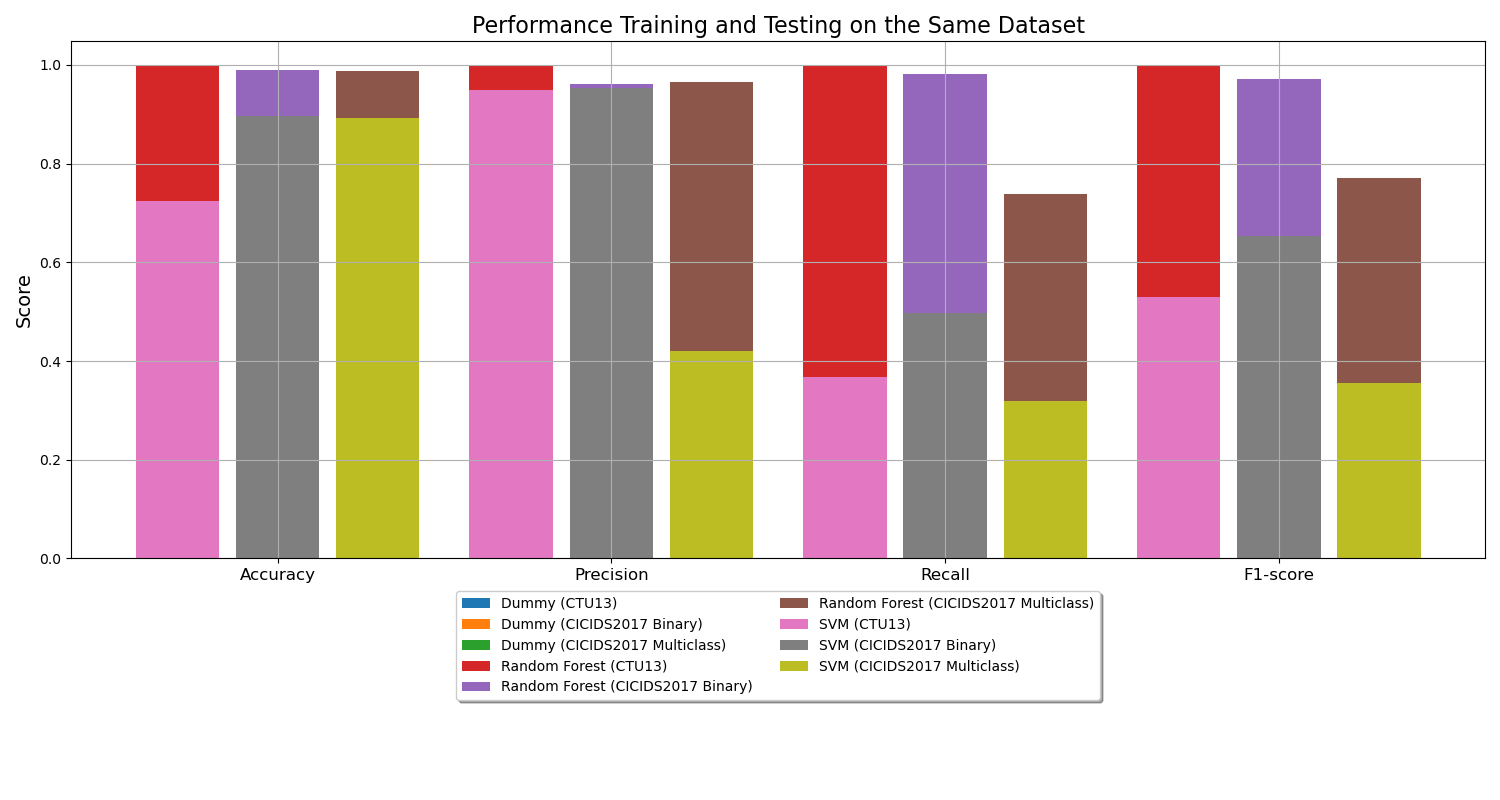
\includegraphics[width=\textwidth]{img/Classifier_Performance_Same_Dataset.png}
\caption{Classifiers' performance on the same datasets.}\label{fig:classifier_performance_same_dataset}
\end{figure}

When testing the classifiers' performance on the same dataset they were trained on, we noted some promising results. The Random Forest model achieves high-performance metrics across the board on both the CTU13 and CICIDS2017 datasets for binary classification. An accuracy, precision, recall, and F1 score of 0.99 on CTU13 and similar scores on CICIDS2017 (accuracy=0.99, precision=0.96, recall=0.98, F1=0.97) indicate that the Random Forest classifiers are effectively learning patterns in the data to distinguish between benign and malicious traffic. These results align with the findings of previous studies that have demonstrated the effectiveness of Random Forest classifiers in detecting network attacks, as discussed in Chapter~\ref{chap:relevant-work}, Section~\ref{sec:RandomForestIntrusion}.

For multi-class classification on CICIDS2017, the Random Forest model still performs respectably with an F1 score of 0.78 (accuracy=0.99, precision=0.90, recall=0.76). While there is room for improvement to reach deployment-level performance, the model demonstrates clear learning compared to the dummy classifier baseline of 0.66. Overall, the Random Forest classifiers consistently outperform the dummy baselines when tested on the same datasets that we trained them on, highlighting their ability to learn discriminative patterns in the data, as discussed in Chapter~\ref{chap:background}, Section~\ref{sec:classifiers}.

In contrast, the SVM classifiers underperform compared to both the Random Forest models and even the dummy classifiers in most cases when evaluated on their training datasets. The binary SVM achieves an accuracy of 0.73, precision of 0.96, recall of 0.37, and F1 score of 0.53 on CTU13. We see similar results for the binary SVM on CICIDS2017 (accuracy=0.73, precision=0.96, recall=0.37, F1=0.65). The multi-class SVM on CICIDS2017 reaches an accuracy of 0.89 but has low precision (0.42), recall (0.32) and F1 (0.35). These results suggest that the current SVM implementations struggle to effectively learn distinguishing patterns, even on the datasets we trained them on. This contrasts with the findings of previous studies that have demonstrated the effectiveness of SVM classifiers in network intrusion detection, as discussed in Chapter~\ref{chap:relevant-work}, Section~\ref{sec:SVMIntrusion}. Improvements to the models will likely be needed, as discussed further in Chapter~\ref{chap:conclusion-future-work}.

\subsection{Feature Importance Analysis on Same Dataset}\label{subsec:feature-importance-analysis-same-dataset}

To better understand how the Random Forest models are making their predictions, we analyse the SHAP (SHapley Additive exPlanations) values. SHAP is an explainable AI technique that assigns importance scores to each feature for a given prediction, providing insight into the model's decision-making process, as discussed in Chapter~\ref{chap:background}, Section~\ref{sec:explainable}.
The appendix listing~\ref{chap:feature-list} provides a guide to interpreting the SHAP value graphs provided in this section.

\subsubsection{Random Forest Model on CTU13}\label{subsec:rf-ctu13}

\begin{figure}[H]
\centering
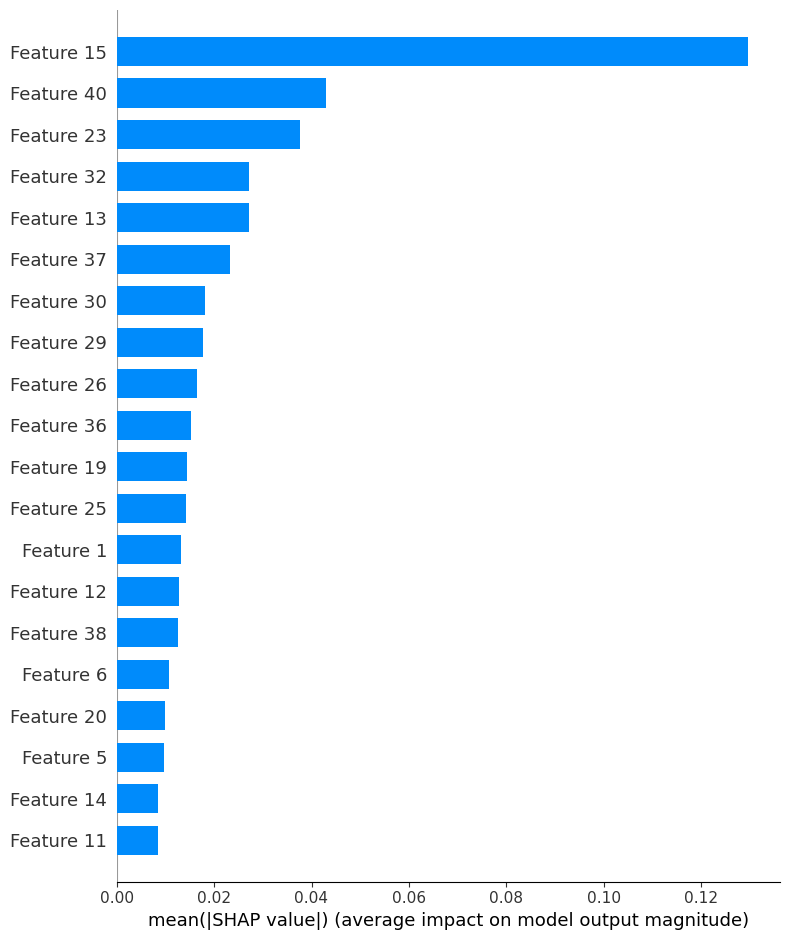
\includegraphics[width=\textwidth]{img/SHAP_RFCTU13_CTU13.png}
\caption{SHAP summary plot for the CTU13 random forest model tested against CTU13 data.}\label{fig:shap_rfc_ctu13_ctu13}
\end{figure}

Figure~\ref{fig:shap_rfc_ctu13_ctu13} shows the SHAP summary plot for the Random Forest model trained and tested on the CTU13 dataset. The features are ranked in descending order of importance, with `Bwd Packet Length Mean' and `Flow IAT Min' having the highest impact on the model's predictions, which suggests that for detecting botnet traffic in CTU13, the size of packets in the backward direction (from destination to source) and the minimum inter-arrival time between packets in a flow are the most informative attributes. Intuitively, this makes sense as botnets often exhibit abnormal communication patterns compared to benign traffic, as discussed in Chapter~\ref{chap:background}, Section~\ref{sec:datasets}.

Other important features include `Fwd Packet Length Min', `Fwd Packet Length Max', and `Fwd IAT Min', indicating that the characteristics of packets in the forward direction (source to destination) also contribute to the model's decision-making. The mix of packet size and inter-arrival time features among the top ranks underscores the importance of both spatial and temporal attributes in identifying botnet behaviour, as highlighted in previous studies discussed in Chapter~\ref{chap:relevant-work}, Section~\ref{sec:RandomForestIntrusion}.

\subsubsection{Random Forest Model on CICIDS2017}\label{subsec:rf-cicids2017}

\begin{figure}[H]
\centering
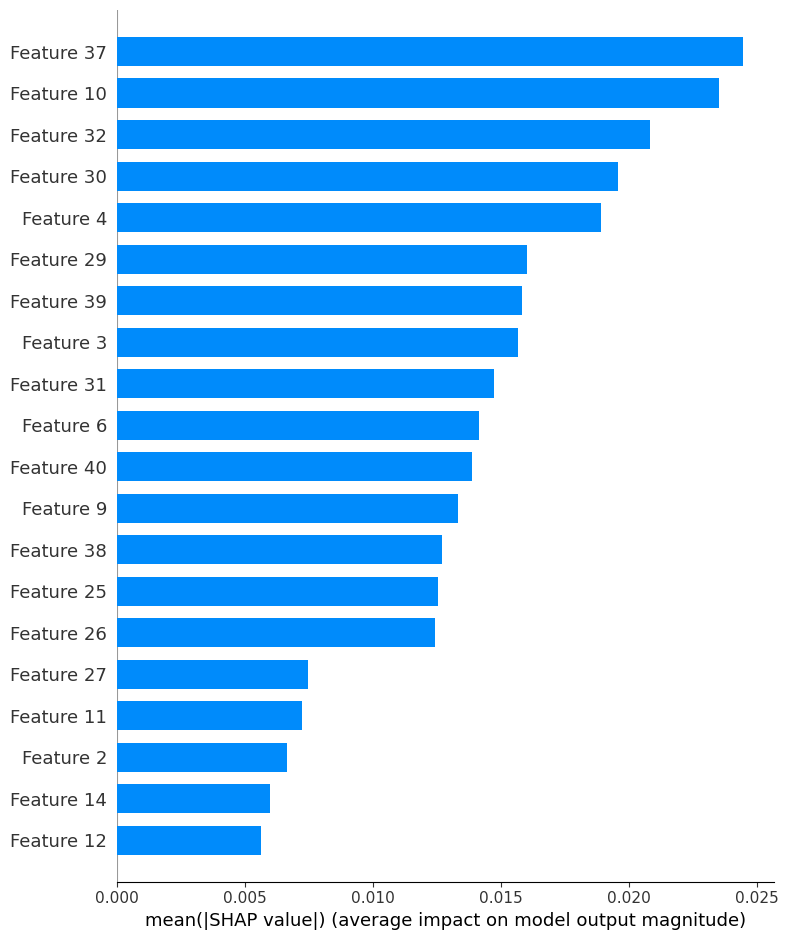
\includegraphics[width=\textwidth]{img/SHAP_RFCICIDS2017_CICIDS2017.png}
\caption{SHAP summary plot for the CICIDS2017 random forest model tested against CICIDS2017 data.}\label{fig:shap_rfc_cicids2017_cicids2017}
\end{figure}

Moving to the Random Forest model trained and evaluated on CICIDS2017 (Figure~\ref{fig:shap_rfc_cicids2017_cicids2017}), we see a somewhat different ranking of important features. Here, `Fwd Packet Length Max' and `Average Packet Size' are the top two contributors, followed by `Bwd Packet Length Std' and `Flow Duration'. The emphasis on packet size attributes, especially in the forward direction, points to the discriminative power of these spatial features for the types of attacks in CICIDS2017, as discussed in Chapter~\ref{chap:background}, Section~\ref{sec:datasets}.

The high rank of `Average Packet Size' is particularly interesting, as it suggests that deviations from standard packet size profiles strongly indicate malicious activity in this dataset. The inclusion of `Flow Duration' among the top features also highlights the relevance of temporal characteristics, as attack flows may exhibit abnormal durations compared to benign ones. These findings align with the observations from previous studies that have analysed the importance of different features in the CICIDS2017 dataset, as discussed in Chapter~\ref{chap:relevant-work}, Section~\ref{sec:RandomForestIntrusion}.

The differences in feature importance between CTU13 and CICIDS2017 underscore the variability in discriminative attributes across datasets. This observation motivates the need to study model transferability, as the most informative features for one dataset may not directly translate to another, addressing RQ1 and RQ3, as discussed in Chapter~\ref{chap:specification-design}, Section~\ref{sec:TransferabilityEvaluation}.

\subsection{Performance on Different Datasets}\label{subsec:performance-different-dataset}

\begin{figure}[H]
    \centering
    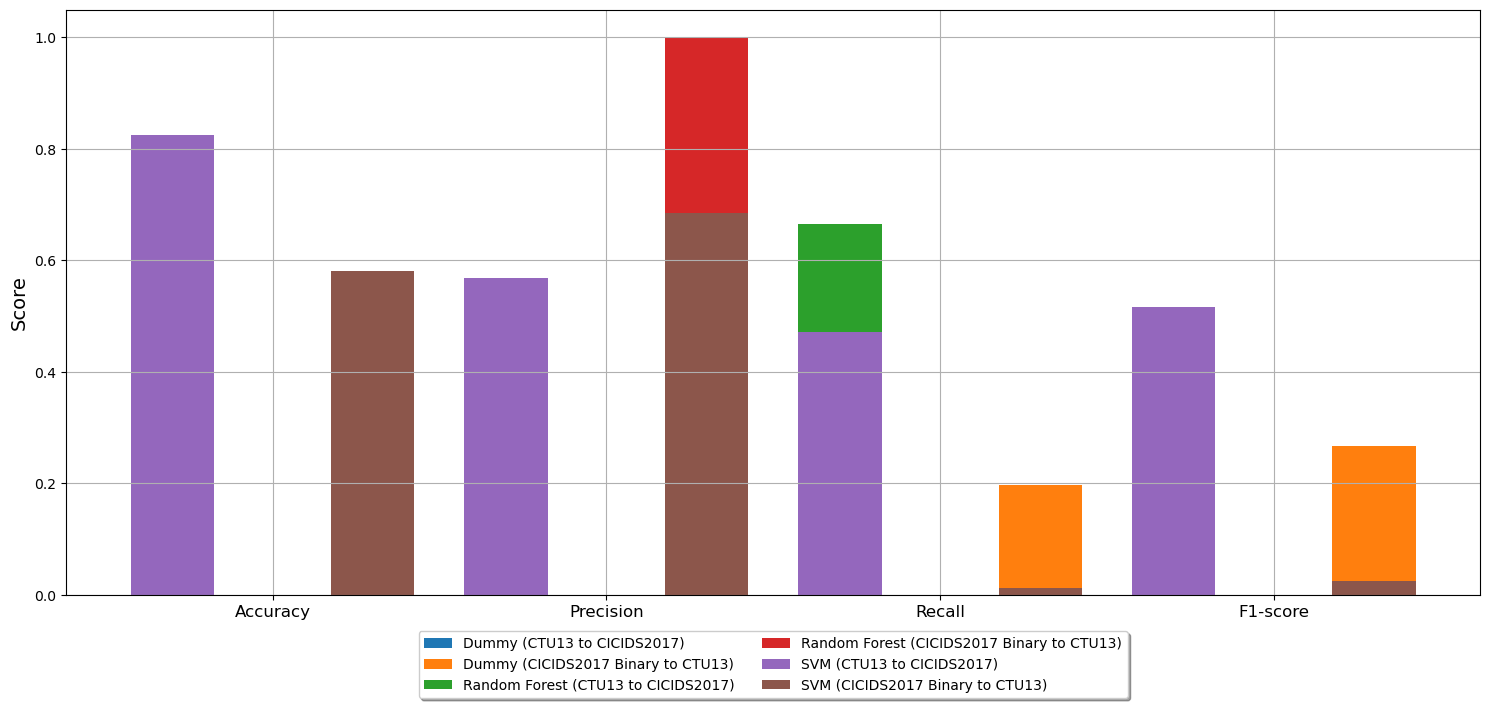
\includegraphics[width=1\textwidth]{img/Classifier_Performance _Across_Datasets.png}
    \caption{Classifiers' Performance across datasets.}\label{fig:classifier_performance_across_dataset}
\end{figure}

To assess the transferability of our trained models, we evaluate their performance when applied to a different dataset than the one we trained them on, as shown in Figure~\ref{fig:classifier_performance_across_dataset}. We observed a substantial drop in performance across all metrics for the Random Forest model trained on CICIDS2017 and tested on CTU13. The accuracy falls to 0.58 and precision to 0.65, while recall and F1-score drop sharply to 0.02 and 0.04, respectively. These results indicate that the patterns learned by the Random Forest on CICIDS2017 do not directly translate to effective botnet detection on CTU13, highlighting the challenges of transferring machine learning models across network intrusion datasets, as discussed in Chapter~\ref{chap:relevant-work}, Section~\ref{sec:ChallengesLimitations}.

The poor recall, in particular, suggests that the model is struggling to identify a significant fraction of the actual botnet traffic in CTU13 when applied out-of-context, which could be due to differences in the statistical profiles of attacks between the datasets, as well as potential overfitting of the Random Forest to CICIDS2017-specific patterns during training. These findings underscore the impact of dataset biases and the importance of representative training data for building robust intrusion detection models, addressing RQ2, as discussed in Chapter~\ref{chap:specification-design}, Section~\ref{sec:TransferabilityEvaluation}.

Interestingly, the SVM models show better transferability in some instances, although they are still underperforming relative to their training dataset baselines. For instance, the SVM trained on CTU13 and evaluated on CICIDS2017 achieves an accuracy of 0.83, precision of 0.57, recall of 0.49, and F1 score of 0.53. While these metrics are lower than the corresponding dummy classifier results on CICIDS2017, they represent an improvement over the SVM's performance on its original CTU13 dataset.

According to the results, the SVM on CTU13 has learned decision boundaries more transferable to CICIDS2017 than the Random Forest model has learned for the opposite direction. Nevertheless, the performance score remains suboptimal, as evidenced by the precision-recall balance that shows many false positives and negatives. These findings highlight the challenges associated with the dynamic nature of network traffic and the evolution of attack patterns, as discussed in Chapter~\ref{chap:relevant-work}, Section~\ref{sec:ChallengesLimitations}.

These transferability results underscore the challenges of applying machine learning models trained on one network intrusion dataset to another. Differences in data distributions, attack types, and feature profiles can significantly degrade cross-dataset performance. Overcoming these limitations will require techniques such as transfer learning, domain adaptation, and more robust feature engineering to improve model generalisation, as discussed in Chapter~\ref{chap:conclusion-future-work}, Section~\ref{chap:conclusion-future-work}.

\subsection{Feature Importance Analysis on Different Datasets}\label{subsec:feature-importance-analysis-different-datasets}

To gain further insight into the transferability challenges, we examine the importance of the SHAP feature for the models when applied to different datasets. The appendix listing~\ref{chap:feature-list} provides a guide to interpreting the SHAP value graphs provided in this section.

\subsubsection{Random Forest Model on CTU13 Tested on CICIDS2017}\label{subsec:rf-ctu13-cicids2017}

\begin{figure}[H]
\centering
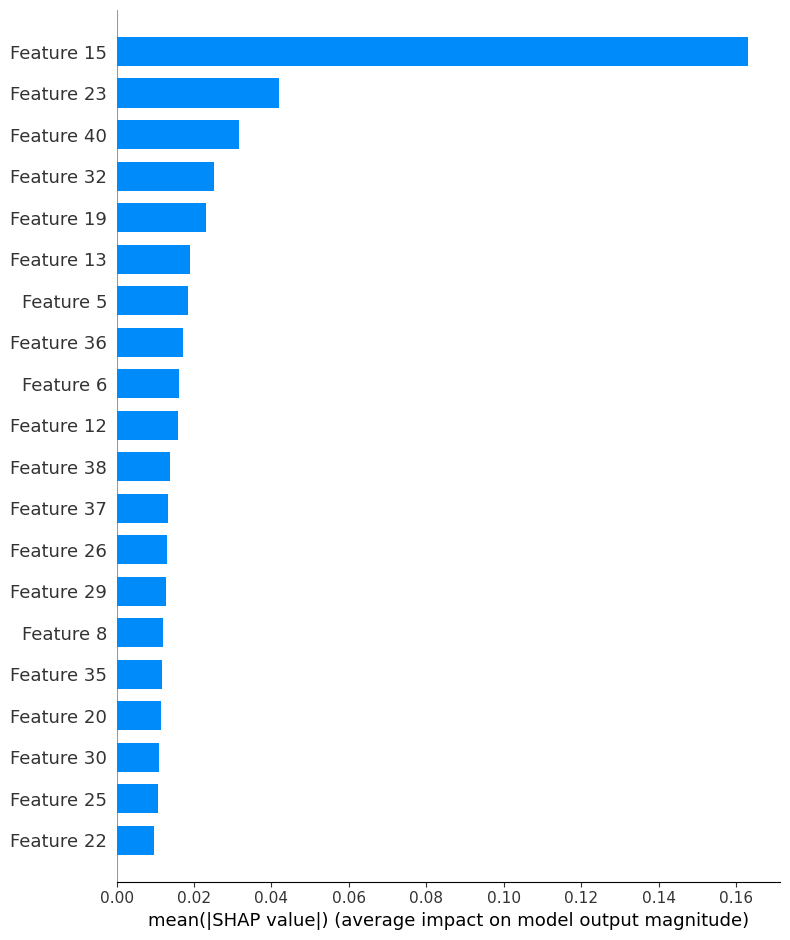
\includegraphics[width=\textwidth]{img/SHAP_RFCTU13_CICIDS2017.png}
\caption{SHAP summary plot for the CTU13 random forest model tested against CICIDS2017 data.}\label{fig:shap_rfc_ctu13_cicids2017}
\end{figure}

Figure~\ref{fig:shap_rfc_ctu13_cicids2017} shows the SHAP values for the Random Forest model trained on CTU13 when applied to CICIDS2017. Comparing this to the original feature importances on CTU13 (Figure~\ref{fig:shap_rfc_ctu13_ctu13}), we observe a notable shift in the top-ranked features. While `Bwd Packet Length Mean' remains important, other attributes such as `Init Win bytes backward' and `Flow Packets/s' now have a higher impact on the model's predictions for CICIDS2017.

This shift suggests that the model relies on different features to make decisions on the new dataset, likely due to differences in the traffic's statistical profiles. The high rank of `Init Win bytes backward', which represents the total number of bytes sent in the initial window in the backward direction, may indicate that this feature better discriminates between attack and benign flows in CICIDS2017 compared to CTU13.

Even with the features' altered importance due to the domain shift observed in CICIDS2017, the effectiveness of the model's classification remains uncertain. The changes merely highlight the model's decision-making process's susceptibility to disruption when applied to data that differs significantly from the training distribution. These findings underscore the importance of addressing transferability issues to enhance the robustness of machine learning models, as discussed in Chapter~\ref{chap:conclusion-future-work}, Section~\ref{chap:conclusion-future-work}.

\subsubsection{Random Forest Model on CICIDS2017 Tested on CTU13}\label{subsec:rf-cicids2017-ctu13}

\begin{figure}[H]
\centering
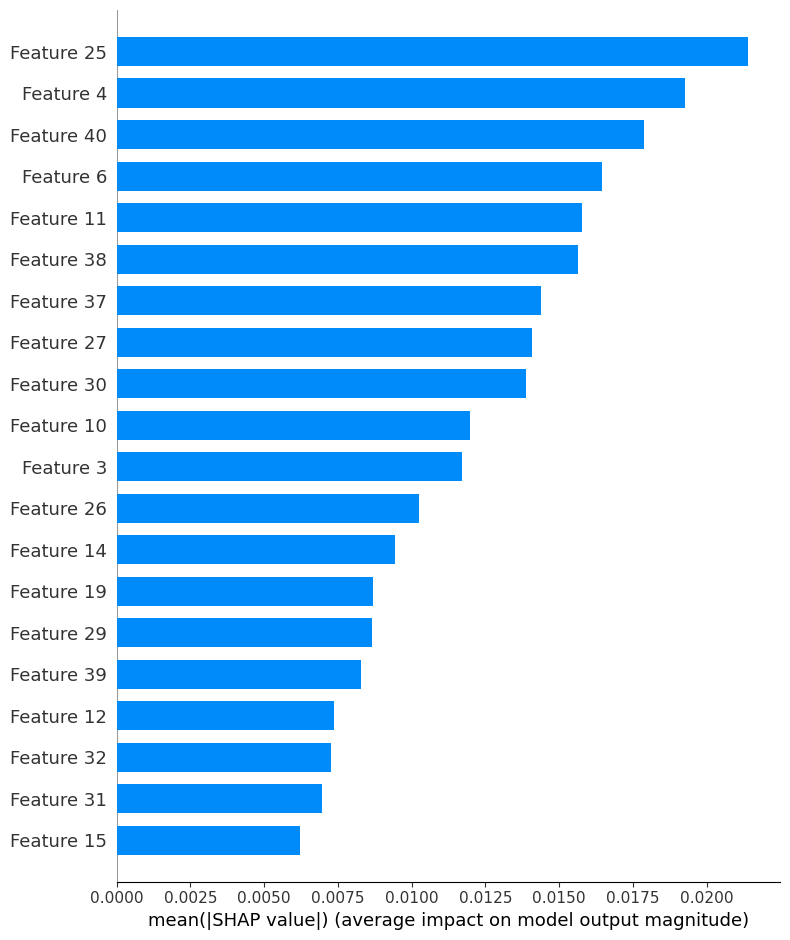
\includegraphics[width=\textwidth]{img/SHAP_RFCICIDS2017_CTU13.png}
\caption{SHAP summary plot for the CICIDS2017 random forest model tested against CTU13 data.}\label{fig:shap_rfc_cicids2017_ctu13}
\end{figure}

Finally, Figure~\ref{fig:shap_rfc_cicids2017_ctu13} presents the feature importances for the Random Forest trained on CICIDS2017 when tested on CTU13. Again, we see a reordering of the top features compared to the model's original dataset (Figure~\ref{fig:shap_rfc_cicids2017_cicids2017}). `Bwd Packet Length Std' and `Fwd IAT Total' now have the highest impact, displacing `Fwd Packet Length Max' and `Average Packet Size'.

This reordering indicates that the model is picking up on different signals in the CTU13 data, emphasising backward packet length variation and forward inter-arrival times. However, as with the CTU13 model on CICIDS2017, these shifted importances align with poor overall performance, underscoring the challenge of directly applying models to new datasets, as discussed in Chapter~\ref{chap:relevant-work}, Section~\ref{sec:ChallengesLimitations}.

The analysis of SHAP values for models applied to different datasets provides valuable insights into the transferability of learned patterns and the most relevant features for detecting specific types of attacks across datasets, addressing RQ3, as discussed in Chapter~\ref{chap:specification-design}, Section~\ref{sec:TransferabilityEvaluation}. The observed shifts in feature importance and the corresponding impact on model performance highlight the challenges posed by dataset biases and the limitations of directly applying models across datasets, as discussed in Chapter~\ref{chap:relevant-work}, Section~\ref{sec:ChallengesLimitations}.

These findings emphasise the need for more advanced techniques, such as transfer learning, domain adaptation, and robust feature engineering, to improve the transferability and generalisation capabilities of machine learning models in the context of network intrusion detection, as discussed in Chapter~\ref{chap:conclusion-future-work}, Section~\ref{chap:conclusion-future-work}. By addressing these challenges and developing more adaptable and interpretable models, we can work towards more practical and reliable machine learning-based network intrusion detection systems that effectively detect and respond to evolving cyber threats across diverse network environments.